% Created 2024-01-01 Mon 19:45
% Intended LaTeX compiler: pdflatex
\documentclass{article}
\usepackage[utf8]{inputenc}
\usepackage[T1]{fontenc}
\usepackage{graphicx}
\usepackage{longtable}
\usepackage{wrapfig}
\usepackage{rotating}
\usepackage[normalem]{ulem}
\usepackage{amsmath}
\usepackage{amssymb}
\usepackage{capt-of}
\usepackage{hyperref}
\author{Keith Butler (20089137)}
\date{\today}
\title{}
\begin{document}

\tableofcontents

\newcommand{\gameName}{Robotic Rebellion}
\newcommand{\shortDescription}{
Robotic Rebellion is a 3D bullet hell action roguelike set in a post robot uprising world.
}

\begin{titlepage}
\begin{center}
\title {
    Game Design Document
    \\
    \vspace{7cm}
    {\huge \gameName}
}

\maketitle
\nopar\noindent\rule{\textwidth}{0.4pt}
\begin{center}\shortDescription\end{center}
\nopar\noindent\rule{\textwidth}{0.4pt}
\vspace{15mm}

\end{center}
\end{titlepage}
\tableofcontents
\section{Declaration}
\label{sec:org4920b6e}
I, Keith Butler, declare that this report is entirely my own work and has not been taken from the work of others. I declare this report has been written entirely in my own words, and all sources used in research are fully acknowledged.
\begin{itemize}
\item Keith Butler (20089137)
\end{itemize}
\section{Game Overview}
\label{sec:org701ab9f}
\subsection{Game Concept}
\label{sec:orgfa6df08}
Robotic Rebellion is a 3D bullet hell action roguelike set in a post robot uprising world where the few remaining humans are hidden in isolated comunities around the world.

A playable demo is available on github: \href{https://github.com/KeithButler-WIT/final\_year\_project}{GitHub - KeithButler-WIT/final\textsubscript{year}\textsubscript{project}}
\subsection{Feature Set}
\label{sec:org8a17784}
\begin{itemize}
\item Fast pace combat
\item Procedural level generation
\item Dynamic difficulty
\item Multiple upgrade paths
\item Boids based ai
\end{itemize}
\subsection{Genres}
\label{sec:org1199312}
3D, Bullet hell, Roguelike, Action, Auto-shooter, Top-down.
\subsection{Target Audience}
\label{sec:org4020dab}

This game is targeted towards people aged 12+ who are looking for a roguelike game that recreates the experience of playing characters such as Engineer in Team Fortress 2(Valve, 2007) and Engineer in Deep Rock Galactic(Ghost Ship Games, 2020).
\subsection{Game Flow Summary}
\label{sec:org9f57405}
Each level will be a fast paced action filled twenty plus minute mission.
\subsection{Look and Feel}
\label{sec:orgf8aa0c5}
The game world is set in a expansive factory compound where almost every surface of the ground is dotted with various forms of machinery.
The game will feature the aesthetic of playstation 1 era retro graphics
\subsection{Project Scope}
\label{sec:orgdd8983e}
\subsubsection{Number of locations}
\label{sec:orgd889448}

6 locations
\subsubsection{Number of levels}
\label{sec:orgd158bf6}

5 levels
\subsubsection{Number of weapons}
\label{sec:orgfd3ca31}
\begin{enumerate}
\item Player Weapons
\label{sec:org3ea8ae1}

Fists \\[0pt]
Crowbar \\[0pt]
Shield
\item Turret Weapons
\label{sec:orgd42d2d5}

4 elemental variations \\[0pt]
2 movement variations \\[0pt]

One elemental variation can be used in tandom with a movement variation to give the player a unique combat experience.
\end{enumerate}
\section{Gameplay and Mechanics}
\label{sec:org60de33d}
\subsection{Gameplay}
\label{sec:org101b3ce}
\subsubsection{Game Progression}
\label{sec:orgedc1568}

As the player progresses through the levels they will unlock points towards the upgrade system that can be used to customise their gameplay style.
\begin{enumerate}
\item Dynamic Difficulty
\label{sec:orgccc6bbc}

Similarly to Risk of Rain 2 (Hopoo Games, 2020).
The difficulty of the game depends on time spent in the level.
The difficulty starts at a low level at the begining of each level, every 3 minutes 0.25 more enemies spawn, each new enemy will also have 0.10\% more health and attack damage. \\[0pt]

This would encourage the player to move quickly and to complete the level before enemies get to difficult for them.
\item Upgrade system
\label{sec:orgd2a7426}
\begin{itemize}
\item 2 Skill trees
\begin{itemize}
\item Turret
\begin{itemize}
\item Increase number of turrets
\item Add mobility
\begin{itemize}
\item Increase move speed
\end{itemize}
\item Hunter mark (ability to make enemies to focus fire on)
\item Bullet pierce
\end{itemize}
\item Player
\begin{itemize}
\item Number of dashes
\item Distance of dashes
\item Delay between dashes
\end{itemize}
\end{itemize}
\end{itemize}
\end{enumerate}
\subsubsection{Objectives}
\label{sec:orgb13ab08}
Player will have the choice of four objectives prior to selecting a mission.
The choices will be:
\begin{enumerate}
\item Retrieve - The player find an item and brings it back to the spawn point.
\item Defend - The player is tasked with protecting a point on the map for a specific amount of time.
\item Destroy - The player is tasked to attack a specific point on the map.
\item Purge - The player is tasked to kill a specific number of enemies.
\end{enumerate}
\subsection{Mechanics}
\label{sec:orgfa20dbf}
\subsubsection{Physics}
\label{sec:org05b86f5}
Unitys built-in physics engine will be used for the games physics.
The engine ``is an integration of the PhysX engine in close partnership with NVIDIA'' (Unity, n.d.).
\subsubsection{Movement}
\label{sec:org381f800}
\begin{enumerate}
\item General Movement
\label{sec:orgebaa256}

The players movement will be controlled by the WASD keys when using a keyboard or by the left joystick when using a controller. \\[0pt]

For the first 0.5 seconds of movement the player will accelerate up to the max speed.

The max speed of the player is detemined by the weapon that's equipped.
\item Other Movement
\label{sec:orgcb6797b}
\begin{enumerate}
\item Dashing
\label{sec:org1e4cf56}

By pressing the \textbf{Space} button the player enters a 'dash' phase in which the player character is launched in the direction of travel.
This would allow the player to move past enemies or hazards with out being affected by them.
\end{enumerate}
\end{enumerate}
\subsubsection{Objects}
\label{sec:org32fb163}
\begin{enumerate}
\item Picking Up Objects
\label{sec:org6cd2db5}

Pickup items will be picked up when the player collised with the objects
\item Moving Objects
\label{sec:orgab28fff}

Crate and box objects that are marked with yellow paint can be pushed by the player.
As the player is colliding with the moveable objects and is trying to move the boxes into an empt space the players base speed is halved
\end{enumerate}
\subsubsection{Actions}
\label{sec:orgd638caa}
\begin{enumerate}
\item Picking Up, Carrying and Dropping
\label{sec:org8702f79}

Certain items can be picked up by the player.

For the player to pickup items all the player has to do is walk on top of the item and it is automatically picked up.
\end{enumerate}
\subsubsection{Combat}
\label{sec:orgf6b9bca}
The focus of the combat will be placed on the placeable turrents that the player has.
The turrets will target the closest enemy to them distance wise.

The player will be able to use weak attack that's not ideal for dealing with groups of enemies.
The will also have access to a shield that while it cannot directly do damage itself it can knock back groups of enemies allowing the player it to be strategicly used in tandom with the turrets or just as a safely net for the player.
\subsection{Screen Flow}
\label{sec:org4d4128b}
\subsubsection{Screen Flow Chart}
\label{sec:org2dee068}
\begin{center}
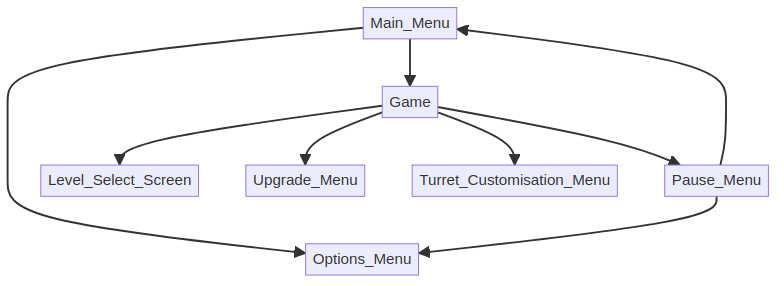
\includegraphics[width=.9\linewidth]{screenflowchart.png}
\end{center}

Flowchart made using (mermaid.js.org, n.d.)
\subsubsection{Screen Descriptions}
\label{sec:org3132821}
\begin{enumerate}
\item Main Menu Screen
\label{sec:org9127116}

\begin{itemize}
\item Continue - Only shown if a save already exists
\item Start
\item Options
\item Quit
\end{itemize}
\item Pause Menu
\label{sec:orge8dcca0}

\begin{itemize}
\item Resume
\item Options
\item Quit
\end{itemize}
\item Options Screen
\label{sec:orgfcd5dcb}

Various gameplay, graphic and accessibility settings can be adjusted here.

Option such as:
\begin{itemize}
\item Graphic quality
\item Lighting
\item Shadows
\item Keybinds
\item Blood
\item Aim Assist
\item Colour blind mode
\end{itemize}
\end{enumerate}
\subsubsection{Game Options}
\label{sec:org7d4acc9}
\begin{itemize}
\item Brightness
\item Volume
\item Aim assist
\end{itemize}
\subsubsection{Replaying and Saving}
\label{sec:orge087666}
The game will save on completion of a level, there will not be any auto saves during missions.
If the player quits the game while in the hub world the game will save before exiting.


Every level can be replayed at any point in the game.
\section{Story, Setting and Character}
\label{sec:org645f0c3}
\subsection{Story and Narrative}
\label{sec:orge1c9e0b}
\subsubsection{Back story}
\label{sec:org86154c9}
A factory is being attacked by evil looking turrets.
A turret falls on an assembly line and lands near the player.
\subsubsection{Game Progression}
\label{sec:org6195c19}
\subsection{Characters}
\label{sec:orgf0c7123}
\subsubsection{Character \#1 The Player}
\label{sec:org872b69b}
\begin{enumerate}
\item Back story
\label{sec:orgab2620d}

Having being born after the robot uprising being ruled over by robots is all this character has every known
but robots are as much a part of life
\item Look
\label{sec:org96aa3f2}

\begin{enumerate}
\item Physical characteristics
\label{sec:orgd0fe9fb}
White jumpsuit.
\item Animations
\label{sec:org189f49b}

\begin{itemize}
\item Walking animation
\item Placing turret animation
\item Dash animation
\end{itemize}
\end{enumerate}
\end{enumerate}
\section{Levels}
\label{sec:orga2f626e}
\subsection{Training Level}
\label{sec:orgd1a4e93}
\subsubsection{Introductory Material}
\label{sec:orgfb2b0a7}
In game cutscene of the player entering the map.
\subsubsection{Objectives}
\label{sec:orgf2ca4cb}
Complete multiple mini tutorials.
\subsubsection{Physical Description}
\label{sec:orgf494331}
\subsubsection{Encounters}
\label{sec:orgcc0434e}
On the fourth mini tutorial the player will encounter the first basic enemies.
The enemy will not be able to attack the player.
This tutorial is to show the player how to attack. \\[0pt]

On the fifth mini tutorial the player will encounter an enemy that is repeatedly doing an attack.
This tutorial is to show the player how to use the dash mechanic to avoid damage.
\subsubsection{Closing Material}
\label{sec:orgfec688b}
In game cutscene of the player exiting the map.
\subsection{Level \#1 : Concrete Jungle}
\label{sec:org6152593}
\subsubsection{Introductory Material}
\label{sec:orga3892c1}
In game cutscene of the player entering the map.
\subsubsection{Objectives}
\label{sec:orgf8eb64c}
Chosen while the player selects the level.
\subsubsection{Physical Description}
\label{sec:orgbfc1ddb}
Random Generation is used to vary the level every time the level is played.
A bleak grey factory setting blinking lights and machinery dot the landscape.

Large open areas.
\subsubsection{Closing Material}
\label{sec:org3023a55}
In game cutscene of the player exiting the map.
\subsection{Level \#2 : Ruined City}
\label{sec:orgd623d11}
\subsubsection{Introductory Material}
\label{sec:org9c1c443}
In game cutscene of the player entering the map.
\subsubsection{Objectives}
\label{sec:orga463188}
Chosen while the player selects the level.
\subsubsection{Physical Description}
\label{sec:org6a8306b}
Random Generation is used to vary the level every time the level is played.
\subsubsection{Closing Material}
\label{sec:org6316590}
In game cutscene of the player exiting the map.
\subsection{Level \#3 : Polluted Waste}
\label{sec:org5ac0185}
\subsubsection{Introductory Material}
\label{sec:org706981c}
In game cutscene of the player entering the map.
\subsubsection{Objectives}
\label{sec:orgf63eb72}
Chosen while the player selects the level.
\subsubsection{Physical Description}
\label{sec:org4b37b5a}
Random Generation is used to vary the level every time the level is played.
Littered with waste and objects that block the players view.
Toxic patches that damage the player and enemies if touched.
\subsubsection{Closing Material}
\label{sec:org0d86124}
In game cutscene of the player exiting the map.
\subsection{Level \#4 : Forgotten Plains}
\label{sec:orgfbf4cc2}
\subsubsection{Introductory Material}
\label{sec:org1d80405}
In game cutscene of the player entering the map.
\subsubsection{Objectives}
\label{sec:org00b201d}
Chosen while the player selects the level.
\subsubsection{Physical Description}
\label{sec:org4ff9a02}
Random Generation is used to vary the level every time the level is played.
An old forgotten town that has been overrun with plant life.
Trees have grown through windows of some buildings.
\subsubsection{Closing Material}
\label{sec:org6f78ea2}
In game cutscene of the player exiting the map.
\section{Interface}
\label{sec:org49d6f40}
\subsection{Visual System}
\label{sec:org74772dd}
\subsubsection{Camera}
\label{sec:org37166d7}
The camera will be snapped to the players position
\subsection{Control System}
\label{sec:org2817073}
The Keys WASD on a keyboard or a controller can be used to controller the player.
\subsection{Help System}
\label{sec:orgf8792e9}
On a new save when a player loads up the game they will be brought to a training level.
In the training level the player will be shown multiple tool tips that explain the mechanics of the game such as dashing, attacking, placing turrets and the basics of a mission loop.
\section{Artificial Intelligence}
\label{sec:org230e117}
\subsection{Enemy AI}
\label{sec:org7d056b4}
Opponent AI will use a modified boids algorithm to simulate a swarm like movement.
The boid model 'is able to simulate complex flocking behavior as a result of coordinated motion by implementing three simple rules that define the steering behavior of each boid' (Mavhemwa and Nyangani, n.d.).

Such an algorithm will allow the enemies to gather in numbers before attacking the player.
This will appear to give the enemies a semblance of strategic thinking from the players point of view.
\section{Technical}
\label{sec:org021312a}
\subsection{Target Hardware}
\label{sec:orgc3644df}
\subsubsection{MINIMUM:}
\label{sec:orga9a22e3}
Requires a 64-bit processor and operating system \\[0pt]
OS : Windows 7 \\[0pt]
Processor: Intel Core 2 Duo \\[0pt]
Memory: 2 GB RAM \\[0pt]
Graphics: DirectX 11 compatible video card (integrated or dedicated with min 512MB memory) \\[0pt]
DirectX: Version 11 \\[0pt]
Storage: 5 GB available space
\subsection{Development hardware and software}
\label{sec:org8cd9ab8}
OS : Arch Linux \\[0pt]
Processor: AMD Ryszn 5 \\[0pt]
Memory: 16 GB RAM \\[0pt]
Graphics: AMD ATI Radeon RX 460 \\[0pt]
DirectX: Version 11 \\[0pt]
\subsection{Game Engine}
\label{sec:orgd3addaf}
Unity Engine
\subsection{Scripting Language}
\label{sec:org00c46bd}
C sharp
\section{Game Art}
\label{sec:org2b7eddb}
\subsection{Concept Art\hfill{}\textsc{ATTACH}}
\label{sec:org73dcdff}
\begin{center}
\includegraphics[width=.9\linewidth]{/home/keith/workspace/org/.attach/0b/dd83cc-2ebb-40b9-8257-99f96610790d/_20231231_144851_b77801de-38a1-43d4-ac8d-f5ebabb81cbc.jpg}
\end{center}

Turret companion concept art, Dall E 3 (2023)



\begin{center}
\includegraphics[width=.9\linewidth]{/home/keith/workspace/org/.attach/0b/dd83cc-2ebb-40b9-8257-99f96610790d/_20231231_144856_b4da1209-befc-4325-8d08-4aa17c511baf.jpg}
\end{center}

Turret companion concept art, Dall E 3 (2023)



\begin{center}
\includegraphics[width=.9\linewidth]{/home/keith/workspace/org/.attach/0b/dd83cc-2ebb-40b9-8257-99f96610790d/_20231231_144902_a860ee91-acf0-4226-ae68-da7c42fec746.jpg}
\end{center}

Turret companion concept art, Dall E 3 (2023)



\begin{center}
\includegraphics[width=.9\linewidth]{/home/keith/workspace/org/.attach/0b/dd83cc-2ebb-40b9-8257-99f96610790d/_20231231_144908_609f7dfd-6a5f-4a4f-bbd2-15297549a970.jpg}
\end{center}

Turret companion concept art, Dall E 3 (2023)



\begin{center}
\includegraphics[width=.9\linewidth]{/home/keith/workspace/org/.attach/0b/dd83cc-2ebb-40b9-8257-99f96610790d/_20231231_171857player 3.jpg}
\end{center}


Player concept art, Dall E 3 (2023)



\begin{center}
\includegraphics[width=.9\linewidth]{/home/keith/workspace/org/.attach/0b/dd83cc-2ebb-40b9-8257-99f96610790d/_20231231_171903player 1.jpg}
\end{center}


Player concept art, Dall E 3 (2023)



\begin{center}
\includegraphics[width=.9\linewidth]{/home/keith/workspace/org/.attach/0b/dd83cc-2ebb-40b9-8257-99f96610790d/_20231231_171915enemy 1.jpg}
\end{center}


Enemy 1 concept art, Dall E 3 (2023)



\begin{center}
\includegraphics[width=.9\linewidth]{/home/keith/workspace/org/.attach/0b/dd83cc-2ebb-40b9-8257-99f96610790d/_20231231_171921enemy 2.jpg}
\end{center}


Enemy 2 concept art, Dall E 3 (2023)
\section{Project Management}
\label{sec:orga4dab4b}
\subsection{Project Methodology}
\label{sec:org271936c}
The scrum methodology will be used.
Scrum is a lightweight framework that helps people, teams and organizations generate value through adaptive solutions for complex problems.
\subsection{Detailed Schedule}
\label{sec:org2953800}
The project will consist of a total of six sprints, each sprint being twelve day long.

\begin{center}
\begin{tabular}{rllll}
Sprint & Start Date & End Date & Deliverables & Prototype Link\\[0pt]
\hline
1 & 01/01/2024 & 14/01/2024 & Prototype 1 & \\[0pt]
2 & 15/01/2024 & 28/01/2024 & Prototype 2 & \\[0pt]
3 & 29/01/2024 & 11/02/2024 & Prototype 3 & \\[0pt]
4 & 12/02/2024 & 25/02/2024 & Prototype 4 & \\[0pt]
5 & 26/02/2024 & 10/03/2024 &  & \\[0pt]
6 & 11/03/2024 & 25/03/2024 & Final Game & \\[0pt]
\end{tabular}
\end{center}
\subsection{Schedule management}
\label{sec:org2ccab92}
\href{https://trello.com/}{Trello} will be used for schedule management and as a scrum/kanban board.

Trello’s look and feel are based on the principles of a Kanban board. (Solomon, n.d.)

Trello has a free tier that makes it an ideal choice for a small team of developers.
\subsection{Version control}
\label{sec:org61d5fd6}
Git/Github will be the version control method used when building this project.
Git has been chosen over Unity Collaborate.
\subsection{Risk Analysis}
\label{sec:org0f0f54d}
\begin{center}
\begin{tabular}{ll}
Risk & Mitigation\\[0pt]
\hline
Project scope too big to be completed in the time frame & Know when and what to scale back if required.\\[0pt]
 & \\[0pt]
\end{tabular}
\end{center}
\subsection{Test Plan}
\label{sec:org3d214dc}
The last 2 days of each sprint will be dedicated to playtests.
\section{Appendices}
\label{sec:org006a716}
\subsection{Credits}
\label{sec:orge07d348}
\href{https://assetstore.unity.com/packages/templates/systems/topdown-engine-89636}{TopDown Engine | Systems | Unity Asset Store}
\subsection{References}
\label{sec:org5491fcf}


\begin{itemize}
\item acaniti, Daniel (February 2018). \href{https://scrumorg-website-prod.s3.amazonaws.com/drupal/2018-02/2018\%20Kanban\%20Guide\%20for\%20Scrum\%20Teams\_0.pdf}{The Kanban Guide for Scrum Teams} (PDF). scrum.org. Retrieved December 28, 2023.
\end{itemize}


\begin{itemize}
\item Ghost Ship Games. (2020). Deep Rock Galactic. [online] Available at: \url{https://www.deeprockgalactic.com/}.
\end{itemize}


\begin{itemize}
\item Hopoo Games, (2020). Risk of Rain. [online] Available at: \url{https://www.riskofrain.com/}.
\end{itemize}
‌

\begin{itemize}
\item Mavhemwa, P. and Nyangani, I. (n.d.). Uniform spatial subdivision to improve Boids Algorithm in a gaming environment. [online] Available at: \url{https://www.ijarnd.com/manuscripts/v3i10/V3I10-1144.pdf} [Accessed 31 Dec. 2023].
\end{itemize}


\begin{itemize}
\item mermaid.js.org. (n.d.). Mermaid | Diagramming and charting tool. [online] Available at: \url{https://mermaid.js.org}.
\end{itemize}


\begin{itemize}
\item Sebastian von Mammen and Jacob, C. (2009). Swarming for Games: Immersion in Complex Systems. Springer eBooks, pp.293–302. \href{https://doi.org/https://doi.org/10.1007/978-3-642-01129-0_33}{doi:https://doi.org/10.1007/978-3-642-01129-0_33}.
\end{itemize}


\begin{itemize}
\item Silva, A.R.D., Lages, W.S. and Chaimowicz, L. (2009). Boids that see. Computers in Entertainment, 7(4), pp.1–20. \href{https://doi.org/https://doi.org/10.1145/1658866.1658870}{doi:https://doi.org/10.1145/1658866.1658870}.
\end{itemize}


\begin{itemize}
\item Solomon, K. (n.d.). What Is Trello Used For? Project Management Software Explained | Trello. [online] blog.trello.com. Available at: \url{https://blog.trello.com/what-is-trello-used-for}.
\end{itemize}


\begin{itemize}
\item Unity, U. (n.d.). Physics solutions for game development | Unity. [online] unity.com. Available at: \url{https://unity.com/solutions/programming-physics}.
\end{itemize}

‌
\begin{itemize}
\item Valve www.teamfortress.com. (2007). Team Fortress 2. [online] Available at: \url{https://www.teamfortress.com/}.
\end{itemize}
\end{document}
